
\section{Sistemas HAR}
\begin{frame}{Sistemas HAR}

\framesubtitle{Aplicaciones de Contexto}

\setbeamercovered{transparent}
\begin{itemize}
\item Aplicaciones cuyo medio de interacci�n es adem�s el contexto.
\end{itemize}

\pause{}
\begin{itemize}
\item El contexto es el estado acerca de la informaci�n
\begin{itemize}
\item f�sica
\item emocional
\item social, entre otros
\end{itemize}
\end{itemize}

\pause{}
\begin{itemize}
\item La computaci�n m�vil y ubicua es sin�nimo de dinamismo en el contexto
\end{itemize}

\pause{}
\begin{itemize}
\item Tipos de contexto comunes en computaci�n m�vil son 
\begin{itemize}
\item la ubicaci�n, 
\item la identidad, 
\item la actividad 
\item y el tiempo
\end{itemize}
\end{itemize}
\end{frame}
%
\begin{frame}[shrink]{Sistemas HAR}

\framesubtitle{Taxonom�a de Actividades Humanas}

\setbeamercovered{transparent}
\begin{columns}[t]



\column{0.5\textwidth}
\begin{itemize}
\item Acciones
\begin{itemize}
\item Gestos
\item Transiciones
\end{itemize}

\pause{}
\item Simples
\begin{itemize}
\item Posturas
\item Ambulatorias
\item Transporte
\end{itemize}

\pause{}
\item Complejas
\begin{itemize}
\item Combinaciones
\item Cotidianas 
\item Gimn�sticas
\item Militares
\end{itemize}

\pause{}
\end{itemize}

\column{0.5\textwidth}
\begin{center}
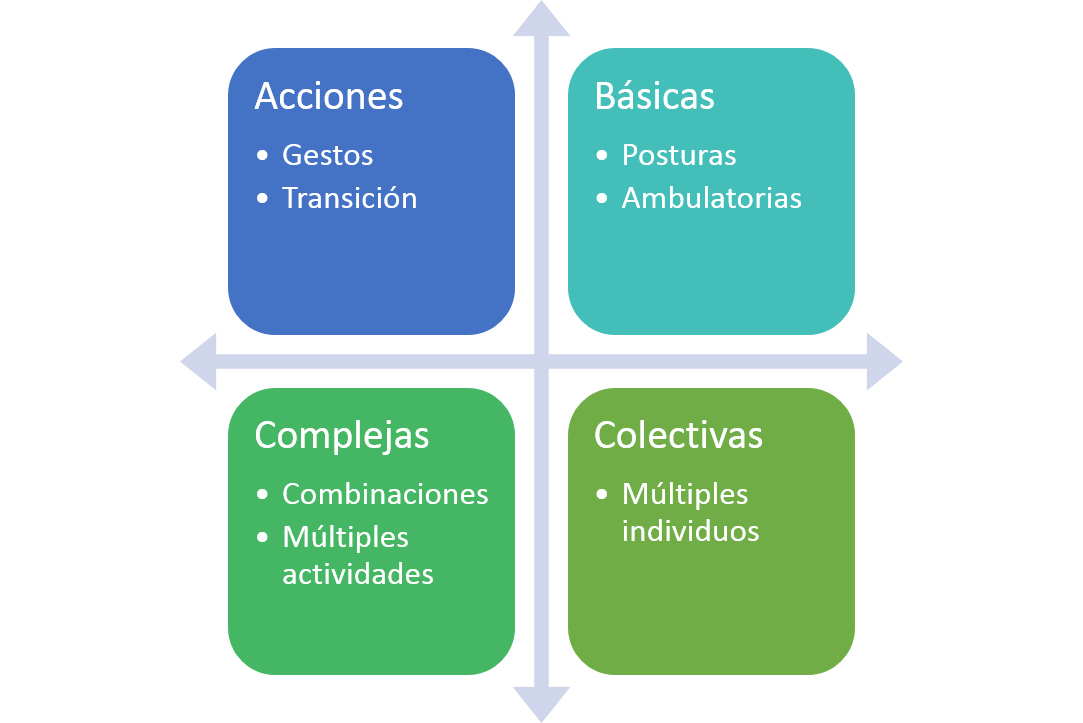
\includegraphics[width=1\columnwidth]{propuesta/graphics/actividades}
\par\end{center}

\end{columns}
\end{frame}
%
\begin{frame}{Sistemas HAR}

\framesubtitle{Prop�sito del sistema}

\setbeamercovered{transparent}
\begin{itemize}[<+->]
\item Proveer un m�dulo para el desarrollo de aplicaciones de contexto. 
\item Reconocer actividades realizadas rutinariamente de diferentes maneras, 
\begin{itemize}
\item por diferentes usuarios y 
\item en diferentes contextos.
\end{itemize}
\item Reconocer las actividades por medio del uso de sensores.
\item Portado oportunamente como atuendo para los usuarios (\emph{Wearable})
\end{itemize}
\end{frame}
%
\begin{frame}{Sistemas HAR}

\framesubtitle{Dise�o del sistema}

\setbeamercovered{transparent}
\begin{itemize}
\item Arquitectura basada en aplicaciones de aprendizaje autom�tico.
\end{itemize}

\pause{}
\begin{itemize}
\item Componentes principales
\begin{itemize}
\item un \structure{recolector} de medidas 
\item un \structure{procesador} de muestras 
\item un \structure{clasificador} de actividades
\end{itemize}
\end{itemize}

\pause{}
\begin{itemize}
\item Metodolog�a operativa
\begin{itemize}
\item Aprendizaje fuera de linea (\emph{off-line})
\item Clasificaci�n en linea (\emph{on-line})
\end{itemize}
\end{itemize}
\begin{center}
\visible<2->{\begin{center}
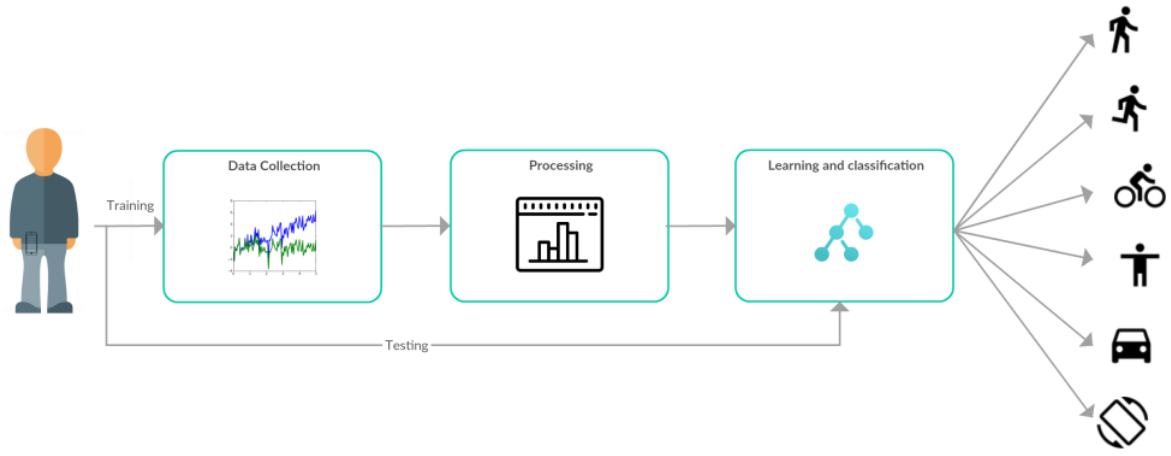
\includegraphics[width=0.75\textwidth]{../capitulo-2/graphics/harsystem2}
\par\end{center}}
\par\end{center}

\end{frame}
%
\begin{frame}{Sistemas HAR}

\framesubtitle{Componentes del sistema}

\setbeamercovered{transparent}
\setlength\columnsep{0pt}
\begin{columns}

\column{0.25\textwidth}
\begin{itemize}
\item Recolector
\begin{itemize}
\item Sensor
\item Registro
\end{itemize}
\end{itemize}

\pause{}
\begin{itemize}
\item Procesador
\begin{itemize}
\item Filtro
\item Extracci�n
\end{itemize}
\end{itemize}

\pause{}
\begin{itemize}
\item Clasificador
\begin{itemize}
\item Aprendizaje
\item Clasificaci�n
\end{itemize}
\end{itemize}

\column{0.75\textwidth}

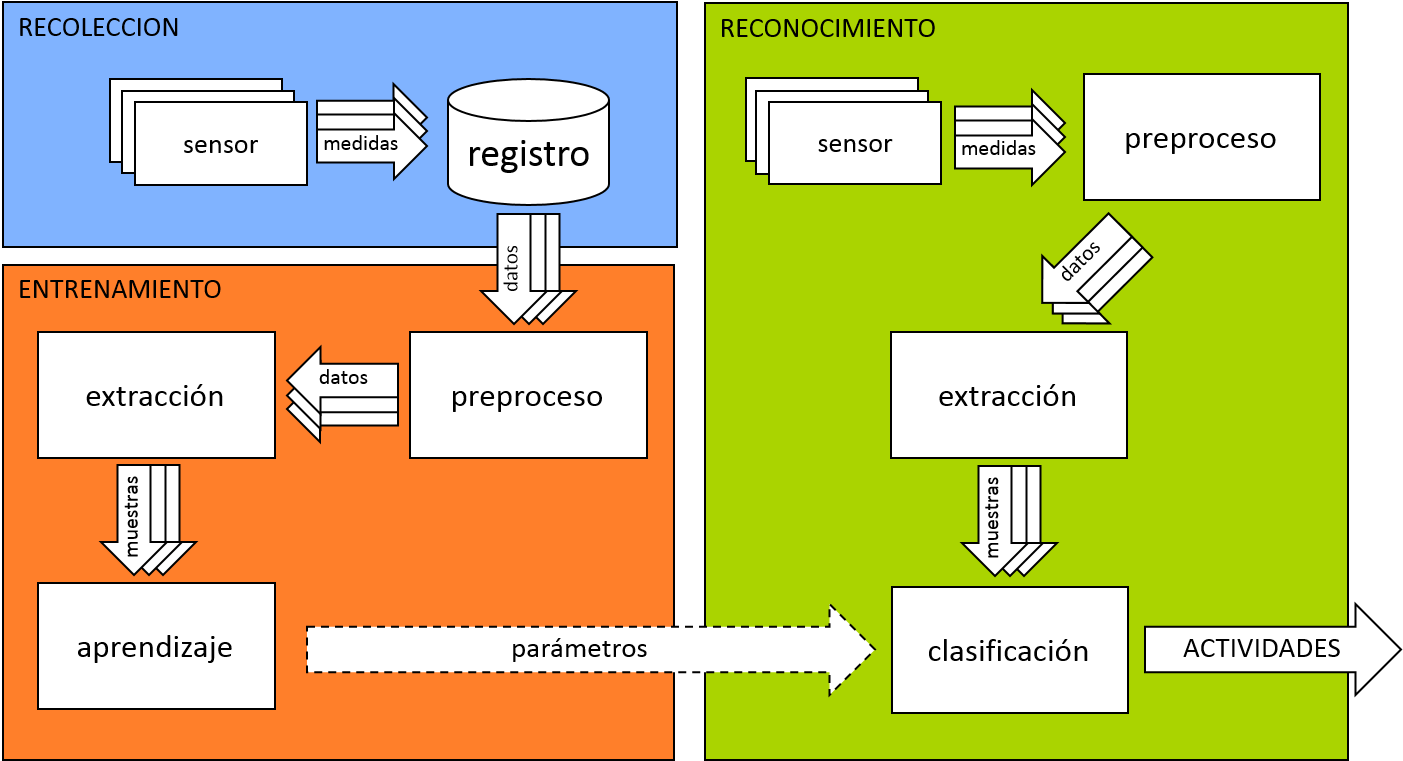
\includegraphics[width=1\columnwidth]{propuesta/graphics/harsystem}
\end{columns}

\end{frame}

